\documentclass{article}
\usepackage{graphicx} % Required for inserting images
\usepackage[utf8]{inputenc}
\usepackage[T2A]{fontenc}
\usepackage{amsmath}
\usepackage{pgfplots}
\usepackage{longtable}
\usepackage{tabularx}
\usepackage{makecell}
\usepackage{array}
\usepackage{indentfirst}
\usepackage{icomma}
\usepackage{geometry}
\usepackage{booktabs}
\usepackage{multirow}
\usepackage{multicol}
\usepackage{float}
\usepackage{diagbox}
\usepackage{gensymb}
\geometry{a4paper, margin=1in}

\renewcommand{\figurename}{Изображение}
\renewcommand{\tablename}{Таблица}

\title{Лабораторная работа №2.04

Определение коэффициента вязкости жидкости
}
\author{Топунов Антон, Z3142}
\date{14.02.2026}

\begin{document}

\maketitle
\clearpage
\section{Цели и задачи}
\subsection{Цели}
\begin{enumerate}
    \item Определение коэффициента внутреннего трения касторового масла методом Стокса.
    \item Проверка справедливости формулы Стокса для шариков разного диаметра.
\end{enumerate}
\subsection{Задачи}
\begin{enumerate}
    \item Измерить размеры шариков с помощью лабораторного микроскопа.
    \item Замерить время равномерного падения шариков в жидкости.
    \item Вычислить значения коэффициентов внутреннего трения для разных шариков и их погрешности.
\end{enumerate}
\section{Теоретическое введение}
Величина силы трения при движении шарика в цилиндре (радиус конечен)
с малой скорость определяется по формуле:
\begin{gather*}
    F=\dfrac{ 6\pi\eta vr}{k } 
\end{gather*}
где
\begin{gather*}
    k=\bigg(1+\dfrac{ 2.4r}{ R} \bigg)^{ -1}
\end{gather*}
\begin{itemize}
    \item $\eta$ - коэффициент вязкости жидкости
    \item $v$ - скорость шарика
    \item $r$ - радиус шарика
    \item $R$ - радиус цилиндра 
\end{itemize}
Коэффициент вязкость жидкость вычисляется по формуле:
\begin{gather*}
    \eta = \frac{ 2}{ 9}\dfrac{r^{ 2}(\rho-\rho_{ 0})}{v}gk
\end{gather*}
\begin{itemize}
    \item $\rho$ - плотность шарика
    \item $\rho_{ 0}$ - плотность жидкости
    \item $g$ - ускорение свободного падения
\end{itemize}

Радиус шарика $r$ можно получить как половина среднего диаметра, который мы получаем с микроскопа:

\begin{gather*}
    r = \alpha \frac{ d}{ 2}
\end{gather*}
\begin{itemize}
    \item $d$ - средний диаметр шарика (в делениях микроскопа)
    \item $\alpha$ - масштаб делений микроскопа
\end{itemize}

Диаметр и средний диаметр:
\begin{gather*}
    d_i = x_2 - x_1\\
    d = \frac{ \sum\limits_{ i=1}^{ N}d_i}{ N} 
\end{gather*}
\begin{itemize}
    \item $x_2$ и $x_1$ - координаты пересечений рисок микроскопа с краями шарика
    \item $N$ - количество измерений
\end{itemize}

Скорость шарика вычисляется по формуле:
\begin{gather*}
    v = \frac{ l}{ t}
\end{gather*}
\begin{itemize}
    \item $t$ - время падения шарика
    \item $l$ - расстояние которое прошел шарик за время $t$
\end{itemize}

Погрешности:
\begin{gather*}
    \Delta{d} = t_{ \alpha, N}\cdot\sqrt{\dfrac{\sum\limits_{ i=1}^{ N} (d_i-d)^2}{N(N-1)}}\\
    \frac{ \Delta{r}}{ r} = \frac{ \Delta{d}}{ d} \\
    \frac{ \Delta{v}}{ v} = \sqrt{\bigg( \frac{ \Delta{l}}{ l} \bigg)^2 + \bigg( \frac{ \Delta{t}}{ t} \bigg)^2}\\
    \frac{ \Delta{k}}{ k} = \frac{ 2.4}{ R}\cdot\sqrt{(\Delta r)^2 + \bigg( \frac{ r\Delta{R}}{ R}\bigg)^2}\\
    \Delta \eta = \eta \cdot\sqrt{\bigg( \frac{ \Delta{v}}{ v} \bigg)^2 + 
        \bigg( \frac{ 2\Delta{r}}{ r} \bigg)^2 + \bigg( \frac{ \Delta{g}}{ g} \bigg)^2 +
        \bigg( \frac{ \Delta{k}}{ k} \bigg)^2 + \dfrac{(\Delta \rho)^2 + (\Delta \rho_0)^2}{(\rho - \rho_0)^2}}
\end{gather*}

\section{Схема установки}
В этой лабораторной работе исследуется движение маленьких шариков в
цилиндрическом объёме жидкости.
Сначала для каждого шарика неколько раз замеряется диаметр а потом шарик
бросают в масло и замеряют время его движения между отмеченными точками
(на расстоянии $l$).

\begin{center}
    
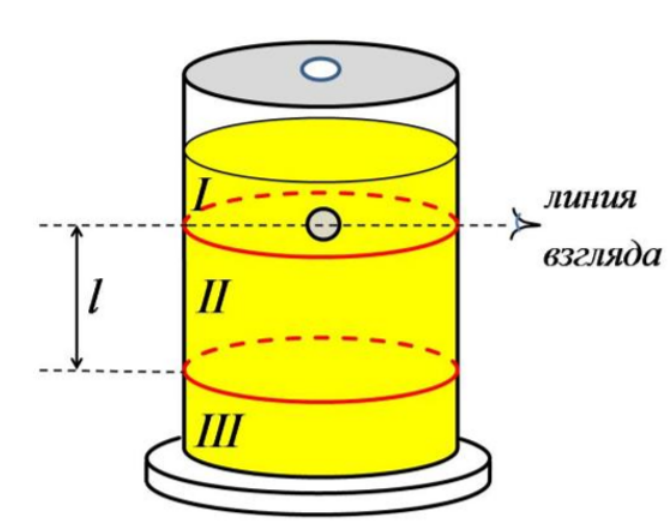
\includegraphics[width=0.7\linewidth]{sc1.PNG}\\
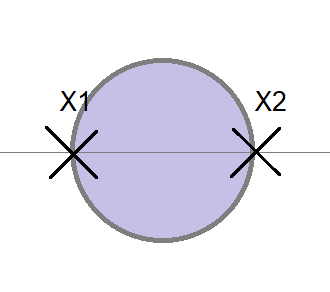
\includegraphics[width=0.5\linewidth]{sc2.png}
\end{center}

\section{Данные прямых измерений, табличные значения}

\begin{table}[H]
   \centering
   \begin{tabular}{|c|c|c|} \hline
       Номер & $x_1$, дел & $x_2$, дел\\ \hline
\multicolumn{3}{|l|}{I}\\ \hline
1 & 0.23 & 7.42\\ \hline
2 & 0.7 & 7.79\\ \hline
3 & 1.07 & 8.13\\ \hline
4 & 1.42 & 8.54\\ \hline
5 & 0.51 & 7.38\\ \hline
\multicolumn{3}{|l|}{II}\\ \hline
1 & 1.52 & 6.11\\ \hline
2 & 1.08 & 5.68\\ \hline
3 & 1.3 & 6.01\\ \hline
4 & 1.45 & 5.98\\ \hline
5 & 1.54 & 6.12\\ \hline
\multicolumn{3}{|l|}{III}\\ \hline
1 & -0.62 & 8.44\\ \hline
2 & -0.41 & 8.74\\ \hline
3 & -0.54 & 8.6\\ \hline
4 & -0.15 & 8.87\\ \hline
5 & -0.53 & 8.55\\ \hline
   \end{tabular}
   \caption{Координаты точек пересечения рисок с краями шариков}
\end{table}

\begin{table}[H]
   \centering
   \begin{tabular}{|c|c|} \hline
    Номер шарика & $t$, с \\ \hline
   I & $11.34$ \\ \hline
   II & $27.75$ \\ \hline
   III & $6.8$ \\ \hline
   \end{tabular}
   \caption{Время падения шариков}
\end{table}

Данные установки:
\begin{itemize}
    \item Расстояние между рисками которое пролетает шарик: $l = (10.2\pm0.1)$ см
    \item Радиус цилиндра с жидкостью: $R = (4.4\pm0.05)$ см
    \item Плотность шариков: $\rho_0 = (7.8\pm0.1) \dfrac{\text{г}}{\text{см}^3}$ 
    \item Плотность жидкости: $\rho = (0.96\pm0.01) \dfrac{\text{г}}{\text{см}^3}$ 
    \item Масштаб делений микроскопа: $\alpha = (0.215 \pm 0.02) \dfrac{\text{мм}}{\text{дел}} $
    \item Погрешность измерения времени: $\Delta t = 0.02$ с
\end{itemize}

Ускорение свободного падения:
\begin{gather*}
    g = (9.82 \pm 0.005) \dfrac{\text{м}}{\text{с}^2}
\end{gather*}

Кожффициент Стьюдента для количества измерений $N = 5$ и доверительной вероятности $0.95$:
\begin{gather*}
    t_{ 0.95, 5} = 2.77
\end{gather*}

\section{Расчёты и графики}
\begin{table}[H]
   \centering
   \begin{tabular}{|c|c|c|c|c|c|} \hline
       & 1 & 2 & 3 & 4 & 5 \\ \hline
       $d_i$, дел & 7.19 & 7.09 & 7.06 & 7.12 & 6.87 \\ \hline
       $d$, дел & \multicolumn{5}{|c|}{$7.07 \pm 0.15$} \\ \hline
       $r$, мм & \multicolumn{5}{|c|}{$0.760 \pm 0.016$} \\ \hline
       $k$ & \multicolumn{5}{|c|}{$0.9602 \pm 0.0009$} \\ \hline
       $v , \dfrac{ \text{мм}}{ \text{с}}$ & \multicolumn{5}{|c|}{$8.99 \pm 0.09$} \\ \hline
       $\eta , \text{Па}\cdot\text{с}$ &  \multicolumn{5}{|c|}{$0.92 \pm 0.04$} \\ \hline 
   \end{tabular}
   \caption{Рассчитанные величичны для шарика I}
\end{table}

\begin{table}[H]
   \centering
   \begin{tabular}{|c|c|c|c|c|c|} \hline
       & 1 & 2 & 3 & 4 & 5 \\ \hline
       $d_i$, дел & 4.59 & 4.60 & 4.71 & 4.53 & 4.58 \\ \hline
       $d$, дел & \multicolumn{5}{|c|}{$4.60 \pm 0.08$} \\ \hline
       $r$, мм & \multicolumn{5}{|c|}{$0.495 \pm 0.009$} \\ \hline
       $k$ & \multicolumn{5}{|c|}{$0.9737 \pm 0.0006$} \\ \hline
       $v , \dfrac{ \text{мм}}{ \text{с}}$ & \multicolumn{5}{|c|}{$3.68 \pm 0.036$} \\ \hline
       $\eta , \text{Па}\cdot\text{с}$ &  \multicolumn{5}{|c|}{$0.968 \pm 0.038$} \\ \hline 
   \end{tabular}
   \caption{Рассчитанные величичны для шарика II}
\end{table}

\begin{table}[H]
   \centering
   \begin{tabular}{|c|c|c|c|c|c|} \hline
       & 1 & 2 & 3 & 4 & 5 \\ \hline
       $d_i$, дел & 9.06 & 9.15 & 9.14 & 9.02 & 9.08 \\ \hline
       $d$, дел & \multicolumn{5}{|c|}{$9.09 \pm 0.07$} \\ \hline
       $r$, мм & \multicolumn{5}{|c|}{$0.977 \pm 0.007$} \\ \hline
       $k$ & \multicolumn{5}{|c|}{$0.9494 \pm 0.0007$} \\ \hline
       $v , \dfrac{ \text{мм}}{ \text{с}}$ & \multicolumn{5}{|c|}{$15.00 \pm 0.15$} \\ \hline
       $\eta , \text{Па}\cdot\text{с}$ &  \multicolumn{5}{|c|}{$0.902 \pm 0.021$} \\ \hline 
   \end{tabular}
   \caption{Рассчитанные величичны для шарика III}
\end{table}

Примеры вычислений:

\begin{gather*}
    d_{ i} = 7.42 - 0.23 = 7.19 \text{ дел}\\
    d = \dfrac{7.19 + 7.09 + 7.06 + 7.12 + 6.87}{5} \approx 7.07\text{ дел}\\
    \Delta d = 2.77 \cdot \sqrt{\frac{ 0.0573}{ 5\cdot4}} \approx 0.15 \text{ дел}\\
    r = 0.215\cdot \frac{ 7.07}{ 2} \approx 0.760 \text{ мм}\\
    \frac{ \Delta{r}}{ r} = \frac{ 0.15}{ 7.07} \approx 0.021\\
    \Delta{r} = r \cdot \frac{ \Delta{r}}{ r} = 0.760 \cdot 0.021 \approx 0.016 \text{ мм}\\ 
    k=\bigg(1+\dfrac{ 2.4\cdot 0.760}{ 44} \bigg)^{ -1} \approx 0.96 \\
    \frac{ \Delta{k}}{ k} = \frac{ 2.4}{ 44}\cdot\sqrt{(0.016)^2 + \bigg( \frac{ 0.760\cdot0.5}{ 44}\bigg)^2}\approx 0.00099\\
    \Delta{k} = k \cdot \frac{ \Delta{k}}{ k} = 0.96\cdot0.00099 \approx 0.0009\\
    v = \frac{ 102}{ 11.34} \approx 8.99 \dfrac{ \text{мм}}{ \text{с}}\\
    \frac{ \Delta{v}}{ v} = \sqrt{\bigg( \frac{ 1}{ 102} \bigg)^2 + \bigg( \frac{ 0.02}{ 11.34} \bigg)^2} \approx 0.0099\\
    \Delta{v} = v \cdot \frac{ \Delta{v}}{ v} = 8.99 \cdot 0.0099 \approx 0.09 \dfrac{ \text{мм}}{ \text{с}}\\
    \eta = \frac{ 2}{ 9}\dfrac{(0.760\cdot10^{-3})^{ 2}(7.8\cdot10^3-0.96\cdot10^3)}{8.99\cdot10^{-3}}9.82\cdot0.96 \approx 0.92 \text{ Па}\cdot\text{с}\\
    \frac{ \Delta{\eta}}{ \eta} = \sqrt{\bigg(0.0099\bigg)^2 + 
        \bigg( 2\cdot0.021 \bigg)^2 + \bigg( \frac{ 0.005}{ 9.82} \bigg)^2 +
        \bigg( 0.00099 \bigg)^2 + \dfrac{(100)^2 + (10)^2}{(6840)^2}} \approx 0.0456\\
    \Delta{\eta} = \eta \cdot \frac{ \Delta{\eta}}{ \eta} = 0.92\cdot0.0456\approx0.04 \text{ Па}\cdot\text{с} 
\end{gather*}

\section{Результаты и выводы}

Коэффициенты вязкостей для шариков получились:
\begin{table}[H]
   \centering
   \begin{tabular}{|c|c|} \hline
       № & $\eta , \text{Па}\cdot\text{с}$ \\ \hline
       I (средний шарик)&   $0.92 \pm 0.04$ \\ \hline
       II (маленький шарик)&  $0.968 \pm 0.038$ \\ \hline
       III (большой шарик)& $0.902 \pm 0.021$ \\ \hline
   \end{tabular}
   \caption{Итоговые значения вязкостей}
\end{table}

Значения вязкостей получились близкими друг к другу и их доверительные интервалы во всех случаях кроме одного пересекаются,
и можно сказать, что они близки к табличному значению вязкости касторового масла при комнатной температуре (около $0.960\text{ Па}\cdot\text{с}$). Относительная погрешность результатов небольшая $\varepsilon_{ \eta} < 5\%$.

Из того, что рассматривались шарики различных размеров, но значения получились почти одинаковыми, можно сделать вывод, что
коэффициент вязкости не зависит от радиуса, а значит метод Стокса справедлив.

\newpage

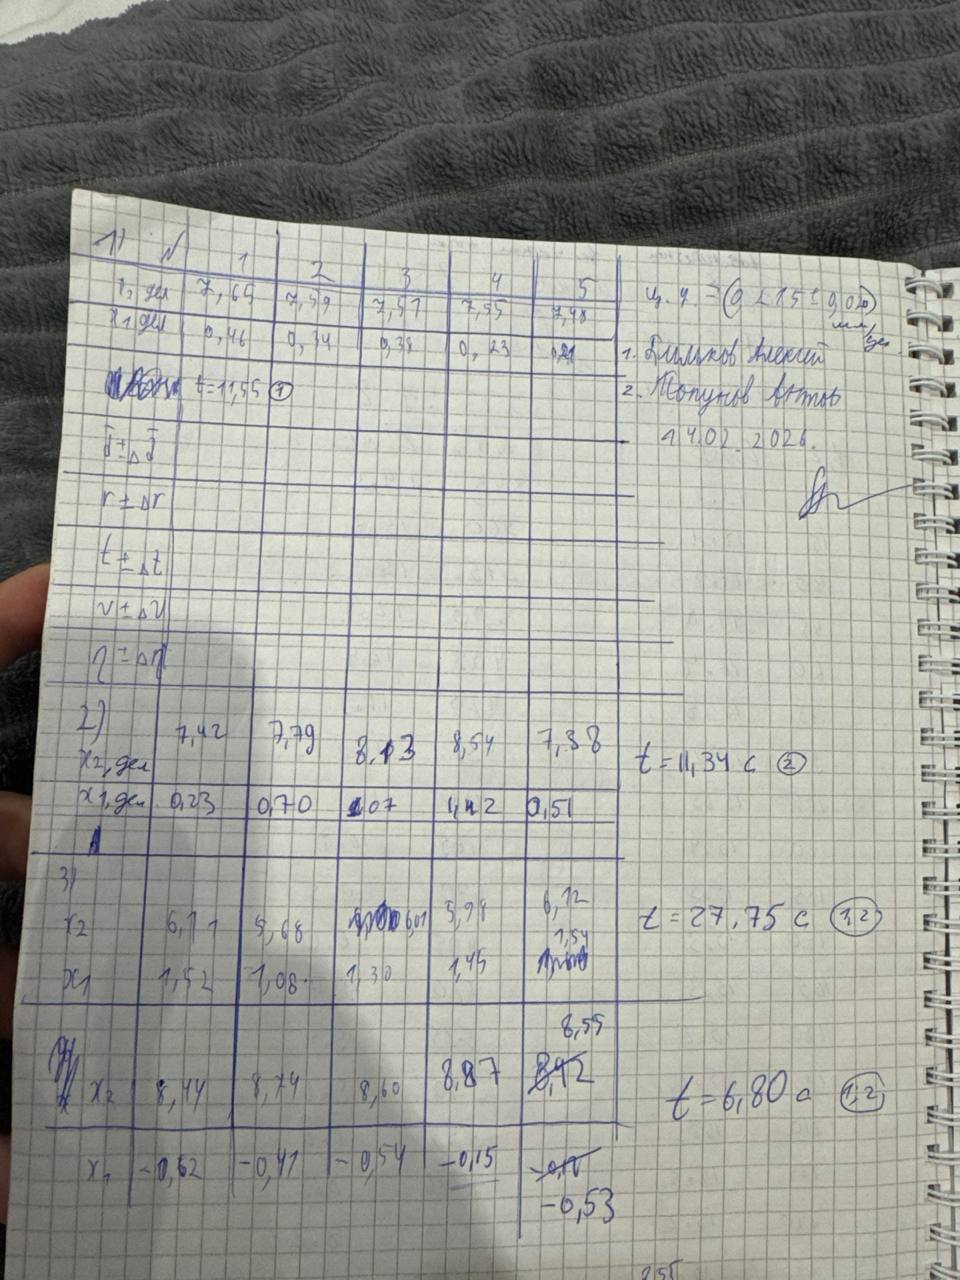
\includegraphics[width=0.95\linewidth]{orig.jpg}\\
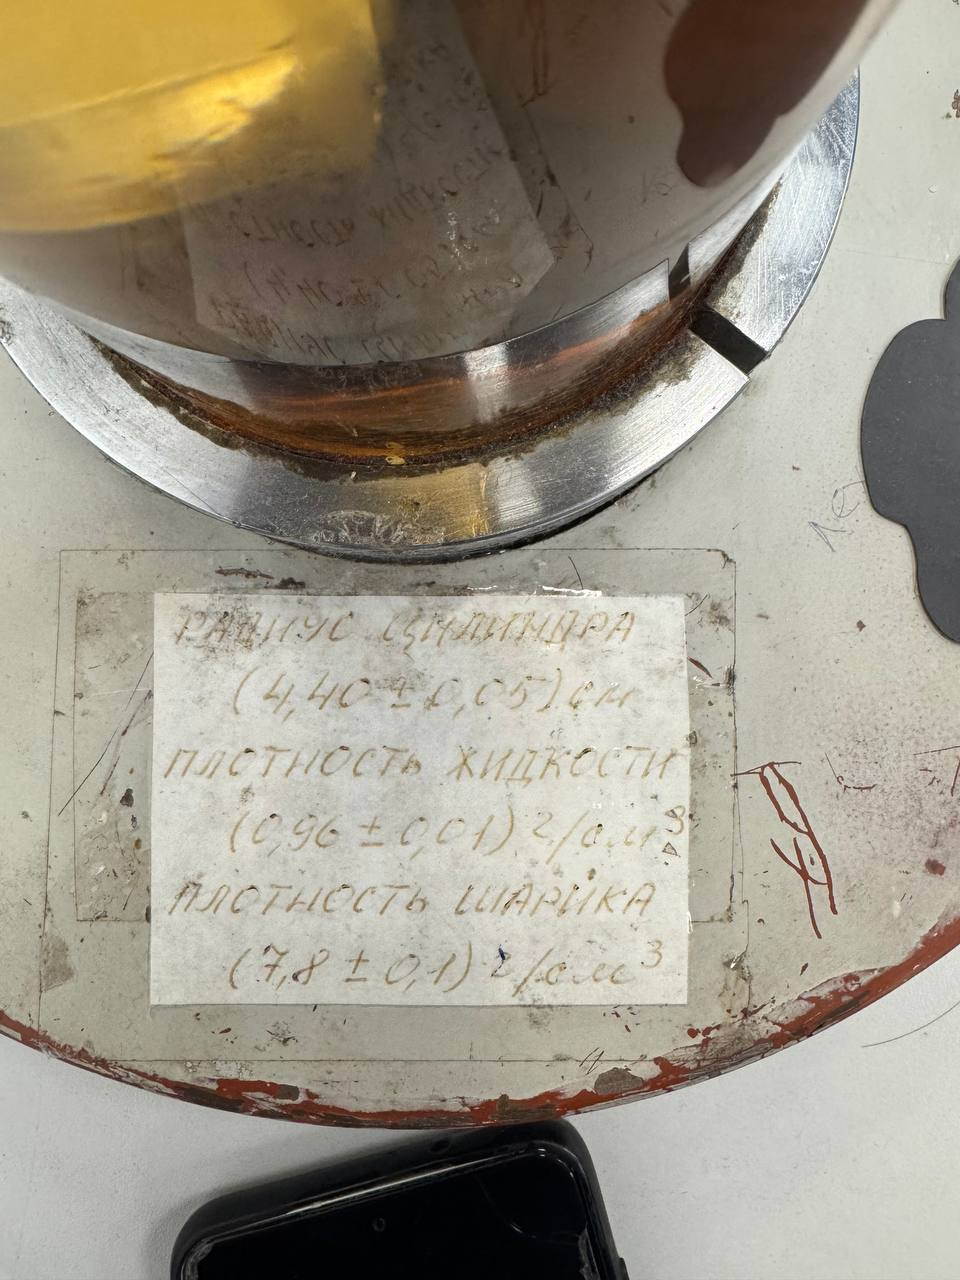
\includegraphics[width=0.5\linewidth]{5246819550622322826.jpg}\\
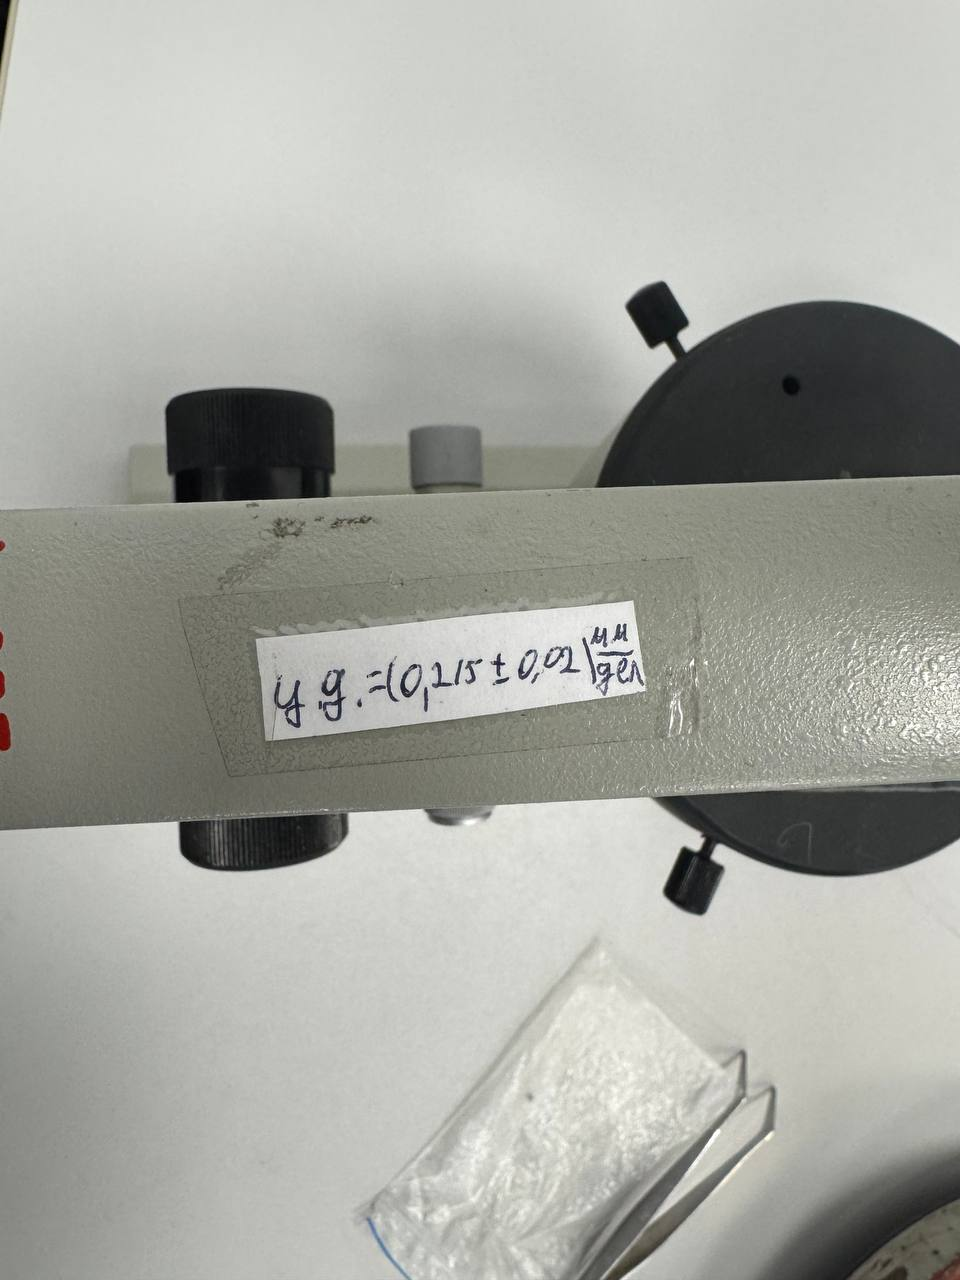
\includegraphics[width=0.5\linewidth]{5246819550622322827.jpg}
\end{document}